%%%%%%%%%%%%%%%%%%%%%%%%%% lecture-14
\begin{frame}[shrink]
  \frametitle{lecture-14 主要内容}
  \framesubtitle{用函数实现模块化程序设计(嵌套与递归)}
  %\tableofcontents[hideallsubsections]
  \tableofcontents
\end{frame}

\section{函数的嵌套调用}

\begin{frame}[shrink,fragile]{函数的嵌套调用}
\begin{columns}[T]
\column{0.4\textwidth}
\begin{lstlisting}
#include<stdio.h>
int a(); int b(); // 函数声明
int main() 
{ 
   int c; // 与a()中的c无关
   c=a(); // 函数调用
   return 0; 
}
\end{lstlisting}
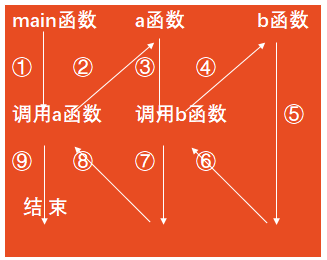
\includegraphics[scale=0.3]{main-a-b}
\column{0.5\textwidth}
\begin{lstlisting}
int a()
{
    int c; // 与main()中的c无关
    ...;
    c=b();// 函数调用
    ...;
    return c;
}
int b()
{
    ...;
    return 10;
}
\end{lstlisting}
\end{columns}
\medskip
\end{frame}


\begin{frame}[shrink,fragile]{例: 求4个整数中的最大者。}
\begin{columns}[T]
\column{0.5\textwidth}
\begin{lstlisting}
#include<stdio.h> 
int max2(int x,int y);
int max4(int a,int b,int c,int d); 
int main() // 主函数
{
   int a=b,c,d;
   scanf("%d%d%d%d",&a,&b,&c,&d);
   printf("较大者=%d\n", max4(a,b,c,d));
   printf("较大者=%d\n", max2(max2(a,b),max2(c,d))); // 等效
   return 0; 
}
\end{lstlisting}
\column{0.4\textwidth}
\begin{lstlisting}
// 定义函数
int max2(int x,int y) // 形式参数
{  
   int z;
   z=x>y ? x : y;
   return z; 
}
int max4(int a,int b,int c,int d)
{
  return max2(max2(a,b),max2(c,d));
}
\end{lstlisting}
\end{columns}
\end{frame}

\section{函数的递归调用}

\begin{frame}[shrink,fragile]{函数的递归调用}
在调用一个函数的过程中又出现直接或间接地调用该函数本身,称为函数的递归调用。
\begin{columns}[T]
\column{0.4\textwidth}
\begin{lstlisting}
// 递推公式: f(0)=0,f(1)=1, 
//     n>1: f(n)=n+f(n-1)
int f(int n) 
{
   int sum;
   if(n==0||n==1) sum=n;
   else sum=n+f(n-1); 
   return sum; 
}
\end{lstlisting}
\column{0.4\textwidth}
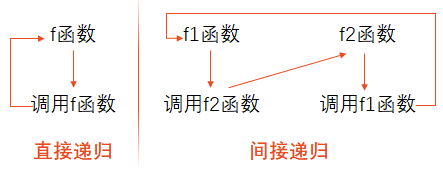
\includegraphics[scale=0.35]{recursion}
\end{columns}
程序中不应出现无终止的递归调用,而只应出现\textbf{有限次数的,有终止的递归调用},这可以用if语句来控制,只有在某一条件成立时才继续执行递归调用;否则就不再继续。
\end{frame}

\begin{frame}[shrink,fragile]{递归调用过程分析(push)}
\begin{lstlisting}
// 递推公式: f(0)=0,f(1)=1, n>1: f(n)=n+f(n-1)
int f(int n) 
{
  int sum;
  if(n==0||n==1) sum=n;
  else sum=n+f(n-1); // 未完成的计算用"栈"存储起来(push)
  return sum; // 函数return前,从"栈"顶取数据,计算,直到"栈"空
}
\end{lstlisting}
系统内部自动维护一个称作``栈"的存储数据的空间,栈是一种``先进后出(FILO)"的数据结构。向栈中存储数据操作称作push, 取出栈顶数据操作称作pop。第一个push的数据,最后一个被pop.
\begin{columns}[T]
\column{0.2\textwidth}<1->
\begin{tabular}{|c|}
	\hline 
	\rowcolor{yellow}f(5)=5+f(4) \\ 
	\hline 
\end{tabular}\\ 
栈[push(n=5)]
\column{0.2\textwidth}<2->
\begin{tabular}{|c|}
	\hline 
	\rowcolor{yellow}f(4)=4+f(3) \\ 
	\hline 
	f(5)=5+f(4) \\ 
	\hline 
\end{tabular}\\ 
栈[push(n=4)]
\column{0.2\textwidth}<3->
\begin{tabular}{|c|}
	\hline 
	\rowcolor{yellow}f(3)=3+f(2) \\ 
	\hline 
	f(4)=4+f(3) \\ 
	\hline 
	\hline 
	f(5)=5+f(4) \\ 
	\hline 
\end{tabular}\\ 
栈[push(n=3)]
\column{0.2\textwidth}<4->
\begin{tabular}{|c|}
	\hline 
	\rowcolor{yellow}f(2)=2+f(1) \\ 
	\hline 
	f(3)=3+f(2) \\ 
	\hline 
	f(4)=4+f(3) \\ 
	\hline 
	\hline 
	f(5)=5+f(4) \\ 
	\hline 
\end{tabular}\\ 
栈[push(n=2)]
\end{columns}
~\\
\end{frame}

\begin{frame}[shrink,fragile]{递归调用过程分析(pop)}
\begin{lstlisting}
// 递推公式: f(0)=0,f(1)=1, n>1: f(n)=n+f(n-1)
int f(int n) 
{
  int sum;
  if(n==0||n==1) sum=n;
  else sum=n+f(n-1); // 未完成的计算用"栈"存储起来(push)
  return sum; // 函数return前,从"栈"顶取数据,计算,直到"栈"空
}
\end{lstlisting}
系统内部自动维护一个称作``栈"的存储数据的空间,栈是一种``先进后出(FILO)"的数据结构。向栈中存储数据操作称作push, 取出数据操作称作pop。第一个push的数据,最后一个被pop.
\begin{columns}[T]
	\column{0.25\textwidth}<4->
	\begin{tabular}{|c|}
		\hline 
		\rowcolor{yellow}f(5)=5+f(4) \\ 
		\hline 
	\end{tabular}\\ 
	栈[pop(n=5)]\\
	f(5)=5+f(4)=15
	\column{0.25\textwidth}<3->
	\begin{tabular}{|c|}
		\hline 
		\rowcolor{yellow}f(4)=4+f(3) \\ 
		\hline 
		f(5)=5+f(4) \\ 
		\hline 
	\end{tabular}\\ 
	栈[pop(n=4)]\\
	f(4)=4+f(3)=10
	\column{0.25\textwidth}<2->
	\begin{tabular}{|c|}
		\hline 
		\rowcolor{yellow}f(3)=3+f(2) \\ 
		\hline 
		f(4)=4+f(3) \\ 
		\hline 
		\hline 
		f(5)=5+f(4) \\ 
		\hline 
	\end{tabular}\\ 
	栈[pop(n=3)]\\
	f(3)=3+f(2)=6
	\column{0.25\textwidth}<1->
	\begin{tabular}{|c|}
		\hline 
		\rowcolor{yellow}f(2)=2+f(1) \\ 
		\hline 
		f(3)=3+f(2) \\ 
		\hline 
		f(4)=4+f(3) \\ 
		\hline 
		\hline 
		f(5)=5+f(4) \\ 
		\hline 
	\end{tabular}\\ 
	栈[pop(n=2)]\\
	f(2)=2+f(1)=3
\end{columns}
~\\
\end{frame}

\begin{frame}[shrink]{例: age(n)}
有5个学生坐在一起,问第5个学生多少岁,他说比第4个学生大2岁。问第4个学生岁数,他说比第3个学生大2岁。问第3个学生,又说比第2个学生大2岁。问第2个学生,说比第1个学生大2岁。最后问第1个学生,他说是10岁。请问第5个学生多大。
~\\
\pause
\[ \text{第n个学生年龄 }
\begin{cases}
age(n)=10         & (n=1)\\
age(n)=age(n-1)+2 & (n>1) 
\end{cases}
\]
\end{frame}

\begin{frame}[shrink,fragile]{例: age(n), 递归调用过程分析(push)}
\begin{lstlisting}
// 递推公式: age(1)=10; n>1: age(n)=age(n-1)
int age(int n) 
{
  int y;
  if(n==1) y=10;
  else y=age(n-1)+2; // 未完成的计算用"栈"存储起来(push)
  return y; // 函数return前,从"栈"顶取数据,计算,直到"栈"空
}
\end{lstlisting}
压栈: push
\begin{columns}[T]
	\column{0.2\textwidth}<1->
	\begin{tabular}{|c|}
		\hline 
		\rowcolor{yellow}age(5)=age(4)+2 \\ 
		\hline 
	\end{tabular}\\ 
	栈[push(n=5)]
	\column{0.2\textwidth}<2->
	\begin{tabular}{|c|}
		\hline 
		\rowcolor{yellow}age(4)=age(3)+2 \\ 
		\hline 
		age(5)=age(4)+2 \\ 
		\hline 
	\end{tabular}\\ 
	栈[push(n=4)]
	\column{0.2\textwidth}<3->
	\begin{tabular}{|c|}
		\hline 
		\rowcolor{yellow}age(3)=age(2)+2 \\ 
		\hline 
		age(4)=age(3)+2 \\ 
		\hline 
		\hline 
		age(5)=age(4)+2 \\ 
		\hline 
	\end{tabular}\\ 
	栈[push(n=3)]
	\column{0.2\textwidth}<4->
	\begin{tabular}{|c|}
		\hline 
		\rowcolor{yellow}age(2)=age(1)+2 \\ 
		\hline 
		age(3)=age(2)+2 \\ 
		\hline 
		age(4)=age(3)+2 \\ 
		\hline 
		\hline 
		age(5)=age(4)+2 \\ 
		\hline 
	\end{tabular}\\ 
	栈[push(n=2)]
\end{columns}
~\\
\end{frame}

\begin{frame}[shrink,fragile]{例: age(n), 递归调用过程分析(pop)}
\begin{lstlisting}
// 递推公式: age(1)=10; n>1: age(n)=age(n-1)
int age(int n) 
{
  int y;
  if(n==1) y=10;
  else y=age(n-1)+2; // 未完成的计算用"栈"存储起来(push)
  return y; // 函数return前,从"栈"顶取数据,计算,直到"栈"空
}
\end{lstlisting}
弹出: pop
\begin{columns}[T]
\column{0.25\textwidth}<4->
\begin{tabular}{|c|}
	\hline 
	\rowcolor{yellow}age(5)=age(4)+2 \\ 
	\hline 
\end{tabular}\\ 
栈[pop(n=5)]\\
age(5)=age(4)+2=18
\column{0.25\textwidth}<3->
\begin{tabular}{|c|}
	\hline 
	\rowcolor{yellow}age(4)=age(3)+2 \\ 
	\hline 
	age(5)=age(4)+2 \\ 
	\hline 
\end{tabular}\\ 
栈[pop(n=4)]\\
age(4)=age(3)+2=16
\column{0.25\textwidth}<2->
\begin{tabular}{|c|}
	\hline 
	\rowcolor{yellow}age(3)=age(2)+2 \\ 
	\hline 
	age(4)=age(3)+2 \\ 
	\hline 
	\hline 
	age(5)=age(4)+2 \\ 
	\hline 
\end{tabular}\\ 
栈[pop(n=3)]\\
age(3)=age(2)+2=14
\column{0.25\textwidth}<1->
\begin{tabular}{|c|}
	\hline 
	\rowcolor{yellow}age(2)=age(1)+2 \\ 
	\hline 
	age(3)=age(2)+2 \\ 
	\hline 
	age(4)=age(3)+2 \\ 
	\hline 
	\hline 
	age(5)=age(4)+2 \\ 
	\hline 
\end{tabular}\\ 
栈[pop(n=2)]\\
age(2)=age(1)+2=12
\end{columns}
~\\
\end{frame}

\begin{frame}[shrink,fragile]{例: $n!$}
\[ n!=\begin{cases}
1 &(n=0,1)\\
n(n-1) &(n>1)
\end{cases} 
\]
\pause
\begin{lstlisting}
double fac(int n) // n!较大,因此函数返回类型设置为double
{
   if(n==0 || n==1) return 1;
   else return n*fac(n-1);
}
int main()                   
{  
   printf("%.0lf\n",fac(2)); // 2
   printf("%.0lf\n",fac(3)); // 6
   printf("%.0lf\n",fac(4)); // 24
   printf("%.0lf\n",fac(20));// 2432902008176640000
   return 0;           
}           
\end{lstlisting}
\end{frame}

\begin{frame}[shrink,fragile]{例: 斐波那契数列}
\[ \begin{cases}
F_n=1 &(n=0,1)\\
F_n=F_{n-1}+F_{n-2} &(n>1)
\end{cases} 
\]
\pause
\begin{lstlisting}
double F(int n) // Fn较大,因此函数返回类型设置为double
{
   if(n==0 || n==1) return 1;
   else return F(n-1)+F(n-2);
}
int main()                   
{  
   int i;
   for(i=0;i<20;i++)
   {
      printf("%d\t",(int)F(i));
      if((i+1)%4==0) printf("\n");	
   } 
   return 0;           
}                            
\end{lstlisting}
\end{frame}

\begin{frame}[shrink,fragile]
求整数$a,b$的最大公约数, 伪代码分析
\begin{lstlisting}
a,b的最大公约数,a=mb+r, m=a/b; r=a%b
while(1)
{
  r = a%b; 
  if(r==0) break; // b就是最大公约数
  else if(b%r==0) break; // r就是最大公约数,因为: n=b/r; r=nb; a=mb+nb=(m+n)b;
  a=b; b=r; // 准备下一轮迭代   
}
\end{lstlisting}
\rule{\textwidth}{1pt} %水平线
\pause
\begin{lstlisting}
  int a,b,r,t;
  scanf("%d%d",&a,&b); // 机试系统不要想当然给提示语句, 除非题目要求
  if(a<b) { t=a; a=b; b=t; } // 交换a,b,使a是较大者
  while(1)
  {
    if(b==0) { t=a; break; }
    r = a%b; 
    if(r==0) {t=b; break;} // b就是最大公约数
    else if(r==1) {t=1; break;} // a,b互质 
    else if(b%r==0) {t=r; break;} // r就是最大公约数,因为: n=b/r; r=nb; a=mb+nb=(m+n)b;
    a=b; b=r; // 准备下一轮迭代   
  }
\end{lstlisting}
\end{frame}

\begin{frame}[shrink,fragile]
求整数$a,b$的最大公约数, 递归实现。
\begin{lstlisting}
// 求a,b的最大公约数(约定a是分子,b是分母)
int gcd(int a, int b) 
{
   int result; 
   if(b==0) result=a; 
   else result=gcd(b,a%b); // b是分子,a%b成为分母 
   return result;
}

int main()                   
{  
  int a,b,t;
  scanf("%d%d",&a,&b);
  if(a<b) // 确保 a > b 
  {
    t=a; a=b; b=t;
  }
  printf("%d\n",gcd(a,b));
  return 0;           
}                   
\end{lstlisting}
\end{frame}

\begin{frame}[shrink,fragile]{例: 数字处理}
编写一个程序,从键盘输入一个非零整数n(0 < n <= 1000000000),对整数n进行如下处理:\\
将整数的各位数字取出来相加,如果结果是一位数则输出该数,否则重复上述过程,直到得到的结果为一位数,并输出该结果。\\
例如:n=456,变换过程如下\\
4+5+6=15\\
1+5=6\\
输出结果为6
\end{frame}

\begin{frame}[shrink,fragile]{例: 数字处理---非递归实现}
\begin{columns}[T]
\column{0.5\textwidth}
\begin{lstlisting}
#include<stdio.h>
int bitsSum(int a);
int main()
{
   int n,sum;
   scanf("%d",&n);
   while(1)
   {
      sum=bitsSum(n);
      if(sum<=9) break;//1位数字
      else n=sum; // 继续下一轮迭代 
    }
    printf("%d\n",sum); 
    return 0;
}
\end{lstlisting}
\column{0.5\textwidth}
\begin{lstlisting}
// 整数a的各位数字之和
int bitsSum(int a)
{
   int sum=0;
   while(a)
   {
      sum += a%10;
      a /= 10;
   }
   return sum;
}
\end{lstlisting}
\end{columns}
~\\
\end{frame}

\begin{frame}[shrink,fragile]{例: 数字处理---递归实现}
\begin{columns}[T]
\column{0.5\textwidth}
\begin{lstlisting}
#include<stdio.h>
int bitsSum(int a);
int bits1(int n);

int main()
{
   int n,sum=0;
   scanf("%d",&n);
   printf("%d\n",bits1(n)); 
   return 0;
} 
\end{lstlisting}
\column{0.5\textwidth}
\begin{lstlisting}
// 整数a的各位数字之和
int bitsSum(int a)
{
   int sum;
   if(a==0) sum=0;  
   else sum=bitsSum(a/10)+a%10;
   return sum;
}
// 确保最后是1位数字
int bits1(int n)
{
   int result;
   result=bitsSum(n);
   if(result<=9) return result;//1位 
   else result=bits1(result);//递归 
}
\end{lstlisting}
\end{columns}
~\\
\end{frame}





